\documentclass[a4paper,12pt,french] {article}

\usepackage{../../../Style}

\renewcommand\tabularxcolumn[1]{m{#1}}

\geometry{bottom=23mm}
\pagestyle{fancy}
\setlength{\headheight}{10mm}
\fancyhead[L]{2021-2022}
\fancyhead[C]{\textbf{Devoir Supplémentaire : Suites et Proportions}}
\fancyhead[R]{\premiere ST2S 2}
\fancyfoot[C]{Page \thepage}

\renewcommand{\baselinestretch}{1.2}

\begin{document}

\rem{L'usage de la calculatrice est autorisé. La propreté et l'orthographe seront prises en compte. Tout le devoir peut être fait sur le sujet.}

Nom: \hfill Prénom: \hfill \

\begin{exercice} \

\vspace{3mm}

\compo[0.6]{
\begin{enumerate}
\item On se donne la suite $v$ définie pour tout $n \in \N$ par $v_n=3-2n$. Compléter:
\begin{itemize}
\item $v_0=$ \dotfill
\item $v_1=$ \dotfill
\item $v_2=$ \dotfill
\item $v_3=$ \dotfill
\item $v_4=$ \dotfill
\item $v_5=$ \dotfill
\item $v_{12}=$ \dotfill
\end{itemize}
\item Représenter la suite $v$ dans le repère ci-contre:
\item Emettre puis prouver une conjecture concernant les variations de $v$. On calculera $v_{n+1}-v_n$:
\end{enumerate}
}
{
\begin{centrer}
\begin{tikzpicture}
\begin{axis}[
styleglobal,
hauteurproptick,
width=0.8*\linewidth,
xmin=0, xmax= 5.5,
ymin=-12, ymax=4,
xlabel={$n$},
ylabel={$u_n$},
minor x tick num=1,
minor y tick num=1,
xtick distance=1,
ytick distance=2,
label style= {font=\normalsize}
]
\end{axis}
\end{tikzpicture}
\end{centrer}
}

\vspace{6mm}

\points 4

\end{exercice}

\begin{exercice} \

\begin{enumerate}
\item Compléter le schéma suivant:

\noindent \begin{tikzpicture}[scale=1.3]
\node[draw,circle,thick, minimum size=18mm] (W0) at (-3,0) {$u_0=2$};
\node[draw,circle,thick, minimum size=18mm] (W1) at (0,0) {$u_1=\ldots$};
\node[draw,circle,thick, minimum size=18mm] (W2) at (3,0) {$u_2=\ldots$};
\node[draw,circle,thick, minimum size=18mm] (W3) at (6,0) {$u_3=\ldots$};
\node (W4) at (9,0) {$\ldots$};
\draw[->,>=latex,thick] (W0) to[bend left=20] node[midway,above]{$\times 4$, $-6$} (W1);
\draw[->,>=latex,thick] (W1) to[bend left=20] node[midway,above]{$\makebox[2cm]{\dotfill}$} (W2);
\draw[->,>=latex,thick] (W2) to[bend left=20] node[midway,above]{$\makebox[2cm]{\dotfill}$} (W3);
\draw[->,>=latex,thick,dashed] (W3) to[bend left=20] node[midway,above]{$\makebox[2cm]{\dotfill}$} (W4);
\end{tikzpicture}

\item Compléter alors la relation de récurrence suivante: $\left\{ \begin{matrix} u_0=\ldots \\ u_{n+1}= \ldots u_n \ldots \end{matrix} \right.$

\item Soit $w$ une suite telle que $w_0=3$ et pour $n \in \N$, $w_{n+1}=(w_n)^2-n$. Calculer:
\begin{itemize}
\item $w_1=$ \dotfill
\item $w_2=$ \dotfill
\item $w_3=$ \dotfill
\item $w_4=$ \dotfill
\end{itemize}
\item Vrai ou faux? La suite $w$ est décroissante. \makebox[3cm]{\dotfill}
\end{enumerate}

\end{exercice}

\newpage

\begin{exercice}
Voici trois situations et trois calculs. Associer chaque situation à un calcul en imaginant une question.
\begin{enumerate}
\item Un ordinateur coute $450$\euro{}. Un commerçant accorde une remise de $6\%$.
\item La longueur d'une piste d'ULM est $450$m. On l'augmente de $6 \%$.
\item $6 \%$ des 450 pompiers d'une ville ont moins de 20 ans.
\end{enumerate}

\noindent \hfill A. $450 \times 1,06$ \hfill B. $450 \times 0,06$ \hfill C. $450 \times 0,94$ \hfill \

\points 6
\end{exercice}

\begin{exercice}
Un pull rétrécit de $1 \%$ à chaque séchage en machine. Après trois séchages, la longueur des manches est $59.4$ cm. Quelle était cette longueur, en cm, avant les trois séchages? On arrondira au dixième près.

\points 4
\end{exercice}

\begin{exercice}
Une oeuvre d'art est achetée par Karim. Il la revend à Clara en faisant une plus-value de $35 \%$. Clara la revend à son tour à Nicolas en faisant un bénéfice de $16 \%$. Sachant que Nicolas a acheté cette oeuvre $70470$\euro{}, combien Karim l'a-t-il achetée au départ?

\points 5
\end{exercice}

\begin{exercice}[*]
Alexis a placé une somme d'argent au taux de $1.75 \%$, les intérêts étant calculés annuellement et ajoutés au solde du compte. Il affirme: "Si je n'effectue aucun retrait et si le taux ne change pas, le solde de mon compte aura plus que doublé dans 40 ans!"
A-t-il raison? Expliquer.

\points 5
\end{exercice}

\begin{comment}
\begin{exercice}
On se donne la suite $u$ représentée ci-dessous:
\begin{center}
\begin{tikzpicture}
\begin{axis}[
styleglobal,
hauteurproptick,
width=0.9*\linewidth,
xmin=0, xmax= 10,
ymin=-3, ymax=5,
xlabel={$n$},
ylabel={$u_n$},
minor x tick num=1,
minor y tick num=1,
xtick distance=1,
ytick distance=2,
label style= {font=\normalsize},
grid style={densely dashed,line width=0.5pt},
]
\addplot[draw=none,samples=11,domain=(0:10),mark=*] {-0.25*(x-5)^2+4};
\end{axis}
\end{tikzpicture}
\end{center}

\begin{enumerate}

\item Déterminer graphiquement $u_2$ et $u_9$: \dotfill
\item Emettre une conjecture concernant les variations de $u$.

\points 1

\item On définit la suite $v$ telle que pour tout $n \in \N, v_n=9n+7$.
\end{enumerate}

\compo[0.5]
{
\begin{enumerate}[label=\alph{enumi})]
\item Représenter la suite dans le repère ci-contre (pour $n$ allant de $0$ à $5$).
\item Emettre puis prouver une conjecture concernant les variations de $v$. On calculera $v_{n+1}-v_n$:

\points 5
\end{enumerate}
}
{
\begin{center}
\begin{tikzpicture}
\begin{axis}[
styleglobal,
hauteurproptick,
width=0.9*\linewidth,
xmin=0, xmax= 5.5,
ymin=0, ymax=50,
xlabel={$n$},
ylabel={$u_n$},
minor x tick num=1,
minor y tick num=1,
xtick distance=1,
ytick distance=10,
label style= {font=\normalsize}
]
\end{axis}
\end{tikzpicture}
\end{center}
}

\vspace{5mm} \setstretch{1.5}{

\hspace{3mm} \dotfill \

\hspace{3mm} \dotfill}

\end{exercice}
\end{comment}

\end{document}